\documentclass{scrartcl}
\usepackage{riley}
\usepackage{riley-libertine}
\usepackage{tikz}
\usetikzlibrary{calc,intersections,through}
\usepackage[top=.9in,left=.8in,right=.8in]{geometry}

%\setlength{\columnseprule}{1pt}
\usepackage{multicol}
\begin{document}
\begin{multicols*}{2}
  \section{Stereographic}
  \[
    \begin{tikzpicture}[scale=2]
      \draw (-1,0)--(2.2,0);
      \coordinate [label=above:{\(N\)}] (N) at (0,1);
      \draw (0,0) -- (N);
      \node(S) [name path=S, draw, circle through=(N)] at (0,0) {};
      \coordinate [label=above:{\(u\)}] (u) at (2,0);
      \draw [name path=ray] (N)--(u);
      \path [name intersections={of=S and ray, by = P}] coordinate[label=below left:{\((x,y)\)}]() at (P);
      \draw let \p1= (P) in (0,\y1) -- (P);
    \end{tikzpicture}
  \]
  \begin{align*}
    N0u &\sim N(0,y)(x,y) \\
    \vec u&=\frac{\vec x}{1-y} \\
    k&\define 1-y \\
    x &= ku \\
    y^2+x^2 &= 1 \\
    \grayunderbrace{(1-k)^2}{1-2k+k^2} + k^2u^2  &= 1 \\
    (1+u^2)k^2 -2k \cancel{+1} &= \cancel 1 \\
    k &= \frac{2}{1+u^2} \\
    \begin{bmatrix}
      x \\y
    \end{bmatrix}
    &= \frac{1}{1+u^2}
      \begin{bmatrix}
        2u^2 \\
        u^2-1
      \end{bmatrix}
  \end{align*}
  \[
    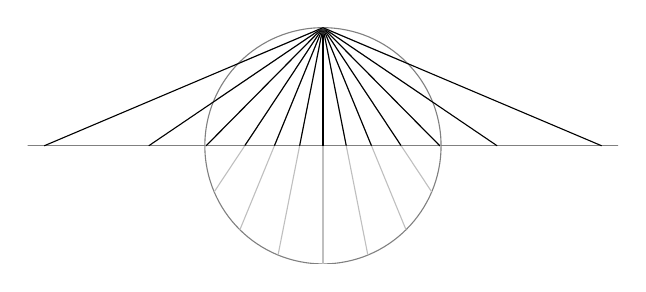
\begin{tikzpicture}[scale=1.5]
      \clip (-2.5,-1) rectangle (2.5,1);
      \draw[gray](-4,0)--(4,0);
      \draw[gray] (0,0) circle (1);
      \foreach \t in {0,.39,...,2.4}
      {
        \draw[lightgray]
        (0,1) -- ({sin(\t r)}, {-cos(\t r)})
        (0,1) -- ({-sin(\t r)}, {-cos(\t r)});
        \draw (0,1) -- ({sin(\t r)/(1+cos(\t r))}, 0)
        (0,1) -- ({-sin(\t r)/(1+cos(\t r))}, 0) ;
      }
    \end{tikzpicture}
  \]
  In one dimension
  \[
    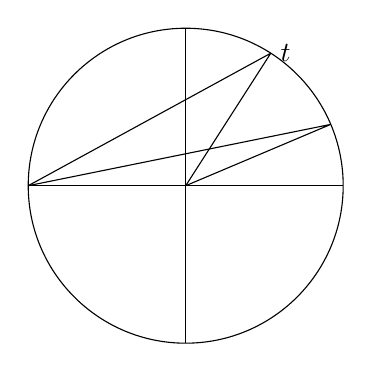
\begin{tikzpicture}[scale=2]
      \draw (0,0) circle (1);
      \draw (0,-1) -- (0,1);
      \draw (-1,0) -- (1,0);
      \def\A{.4}
      \def\B{1}
      \coordinate (P) at ({cos(\A r)},{sin(\A r)});
      \coordinate (P2) at ({cos(\B r)},{sin(\B r)});
      \draw (-1,0) -- (P) (0,0)--(P);
      \draw (-1,0) -- (P2) (0,0)--(P2);
      \node[ right] () at  (P2) {\(t\)};
    \end{tikzpicture}
  \]
  Via projective geometry:
  \begin{align*}
    \begin{bmatrix}
     \cos \sfrac t2 & -\sin \sfrac t2 \\
     \sin \sfrac t2 & \cos \sfrac t2
    \end{bmatrix}
    \begin{bmatrix}
      1 \\ u
    \end{bmatrix}
    &=
      \begin{bmatrix}
        -u\sin\sfrac t2 + \cos \sfrac t2 \\
        u \cos \sfrac t2  + \sin \sfrac t2
      \end{bmatrix} \\
    &\sim
      \begin{bmatrix}
        1 \\
        \dfrac{u \cos \sfrac t2  + \sin \sfrac t2}{-u\sin\sfrac t2 + \cos \sfrac t2}
      \end{bmatrix}
  \end{align*}
  \[
    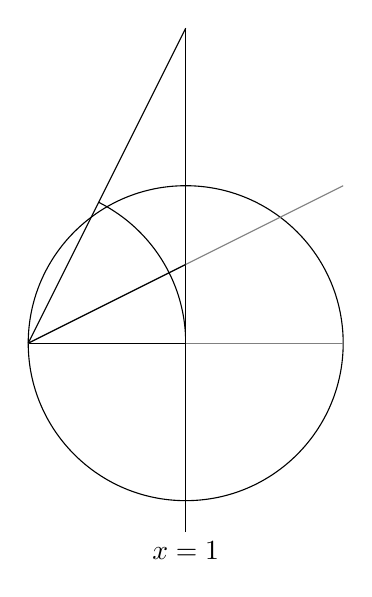
\begin{tikzpicture}[scale=2]
      \draw (1,-1.2) coordinate[label=below:{\(x=1\)}] -- (1,2);
      \draw (1,0) circle (1);
      \draw[gray] (0,0) -- (2,0);
      \draw (0,0) -- (1,0);
      \draw[gray] (0,0) -- (2,1);
      \draw (0,0) -- (1,.5);
      \draw (0,0) -- (1,2);
      \begin{scope}
        \clip (0,0) -- (1,2) -- (1,0) -- cycle;
        \draw (0,0) circle (1);
      \end{scope}
    \end{tikzpicture}
  \]
  \(S^n\)
  \begin{align*}
    \begin{bmatrix}
      \vec x \\y
    \end{bmatrix}
    &\mapsto \frac{1}{u^2+1}
      \begin{bmatrix}
        2\vec x \\ 2y \\ u^2-1
      \end{bmatrix} \\
    &\mapsto \frac{1}{u^2+1}
      \begin{bmatrix}
        1 \\
        & \gamma & -\sigma \\
        & \sigma & \gamma
      \end{bmatrix}
      \begin{bmatrix}
        2x \\ 2y \\ u^2-1
      \end{bmatrix} \\
    &\propto
    \begin{bmatrix}
      2x \\
      2y\gamma -\paren{u^2-1}\sigma \\
      2y\sigma + \paren{u^2-1}\gamma
    \end{bmatrix} \\
    &\mapsto
      \frac{
      \begin{bmatrix}
        2\vec x \\
        2y\gamma - (u^2-1)\sigma
      \end{bmatrix}
}{1- 2y\sigma - \paren{u^2-1}\gamma}
      \shortintertext{Which, for \(S^1\), reduces to}
      &\mapsto \frac{2y\gamma - \paren{y^2-1}\sigma}{1-2y\sigma - (y^2-1)\gamma}
  \end{align*}
  \subsection{the metric}
  \begin{align*}
    F(u) &=
        \frac{1}{u^2+1}
        \begin{bmatrix}
          2u \\
          u^2-1
        \end{bmatrix} \\
    dF(u) &=
            -
            \begin{bmatrix}
              2u \\ u^2-1
            \end{bmatrix}
            \frac{2u^\flat}{\paren{u^2+1}^2}
            +
            \frac{1}{u^2+1}
            \begin{bmatrix}
              2 \\ 2u^\flat
            \end{bmatrix} \\
         &= 2\frac{
           \begin{bmatrix}
             u^2+1 \\ (u^2+1)u^\flat
           \end{bmatrix}
           -
           \begin{bmatrix}
             2uu^\flat \\ (u^2-1)u^\flat
           \end{bmatrix}
           }{\paren{u^2+1}^2} \\
         &=\frac{2}{\paren{u^2+1}^2}
           \begin{bmatrix}
             u^2+1-2uu^\flat \\
             2u^\flat
           \end{bmatrix} \\
    dF(u)(X) &= \frac{2}{\paren{u^2+1}^2}
               \begin{bmatrix}
                 \paren{u^2+1}X - 2 u{u}^\flat{X} \\
                 2 {u}^\flat  X
               \end{bmatrix} \\
    \abs{dF_u(X)}^2 &= \frac{4}{\paren{u^2+1}^4}\paren{
                       \begin{matrix}
                         (u^2+1)^2\abs X^2 \\
                         + \cancel{4 \abs u^2 (u^\flat X)^2} \\
                         -4(\cancel{\abs u^2}\cancel{+1})\paren{X^\flat u}^2 \\
                         + \cancel{4 \paren{u^\flat X}^2}
                       \end{matrix}
                       } \\
         &= \frac{4}{\paren{u^2+1}^2} \abs X^2\\
    \intertext{By dimensional analysis,}
    &= \frac{4 R^4}{\paren{u^2+R^2}^2} \abs X^2\\
      \abs{dF(u)(X)} &= \frac{2 R^2}{ u^2 + R^2}\abs X
  \end{align*}
  When \(R\to\infty\), \(\abs X \mapsto 2\abs X\)
  \[
    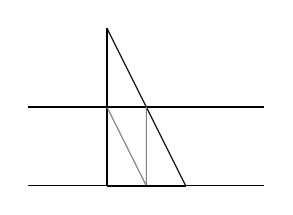
\begin{tikzpicture}
      \draw(0,1) -- (0,-1);
      \draw(-1,0) -- (2,0);
      \draw(-1,-1) -- (2,-1);
      \draw (0,1) -- (1,-1);
      \draw[gray] (.5,0) -- (.5,-1) (0,0) -- (.5,-1);
      \draw[thick] (0,0) -- (.5,0)
      (0,-1)--(.5,-1) (.5,-1)--(1,-1);
    \end{tikzpicture}
  \]
  Single particle lagranian
  \begin{align*}
    S&= \int \frac12  \abs {\dot u}_{F} ^2 \\
     &= \int \frac12 \paren{\frac{4}{\paren{u^2+1}^2}} \abs{\dot u}_{\R^n}^2 \\
     &=\int \grayunderbrace{\frac{2\dot u^2}{\paren{u^2+1}^2}}{L}  \\
    \frac{\partial L}{\partial u}&=\frac{-8\dot u^2u^\flat}{\paren{u^2+1}^3} \\
    \frac{\partial L}{\partial \dot u}&= \frac{4\dot u^\flat}{\paren{u^2+1}^2} \\
    E&= \frac{4\dot u^2 }{\paren{u^2+1}^2} - \frac {2\dot u^2}{\paren{u^2+1}^2} \\
     &= \frac{2\dot u^2}{\paren{u^2+1}^2} = L \\
    \frac{d}{dt}\frac{\partial L}{\partial \dot u}
     &=  \frac{4\ddot u^\flat}{\paren{u^2+1}^2} - \frac{16 \paren{u^\flat \dot u}\dot u^\flat}{\paren{u^2+1}^3} \\
    \frac{d}{dt}\frac{\partial L}{\partial \dot u}-\frac{\partial L}{\partial u}&=\frac{4\ddot u^\flat}{\paren{u^2+1}^2} + \frac{8\dot u^2 u^\flat - 16 u^\flat\dot u \dot u^\flat}{\paren{u^2+1}^3} \\
    0&= \ddot u^\flat - \frac{2u^\flat}{u^2+1}\paren{2  \dot u \dot u^\flat-\dot u^2} \\
    &= \ddot u \grayunderbrace{- \frac{2u\paren{2-\delta}_{\alpha\beta}}{u^2+1}}{\Gamma_{\alpha\beta}} \dot u_\alpha\dot u_\beta
  \end{align*}
  \vfil
  \section{Hyperboloid}
  \[
    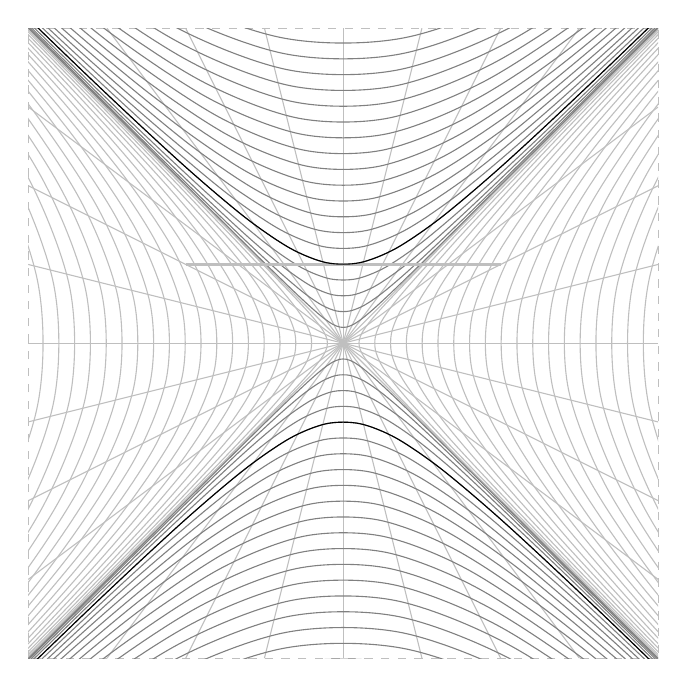
\begin{tikzpicture}
      \draw[dashed,lightgray] (-4,-4) rectangle (4,4);
      \clip                   (-4,-4) rectangle (4,4);
      \foreach \x  in {0,1,...,4}
      \draw[lightgray]
      (0,0) -- (\x,4)
      (0,0) -- (-\x,4)
      (0,0) -- (\x,-4)
      (0,0) -- (-\x,-4)
      (0,0) -- (4,\x)
      (0,0) -- (4,-\x)
      (0,0) -- (-4,\x)
      (0,0) -- (-4,-\x)
      ;
      \foreach \R in {0,.2,...,4}
      {
        \draw[lightgray,samples=20, domain=-4:4,smooth,variable=\t]
        plot ({\R * cosh \t},  {\R * sinh \t})
        plot ({- \R * cosh \t},{\R * sinh \t})
        ;
        \draw[     gray,samples=20, domain=-4:4,smooth,variable=\t]
        plot ({\R * sinh \t}, {\R * cosh \t})
        plot ({\R * sinh \t}, {- \R * cosh \t})
        ;
      }
      \draw[thick,lightgray] (-2,1) -- (2,1);
      \def\R{1}
      \draw[          samples=20, domain=-4:4,smooth,variable=\t]
      plot ({\R * sinh \t}, {\R * cosh \t})
      plot ({\R * sinh \t}, {- \R * cosh \t})
      ;
    \end{tikzpicture}
  \]
  The proper-length metric is positive definite on \(H^+\):
  \begin{align*}
    N &= (1,0) \\
    T_NH^+ &= dt^{-1}(0) \\
    &= \set{
      \begin{bmatrix}
        0 \\ x
      \end{bmatrix}
      : x  \in \R^n
      } \\
    \begin{bmatrix}
      0 \\x
    \end{bmatrix}^\flat
    \begin{bmatrix}
      0 \\x
    \end{bmatrix}
    &=
      \begin{bmatrix}
        -0 & x^\flat
      \end{bmatrix}
      \begin{bmatrix}
        0 \\ x
      \end{bmatrix} \\
    &= \abs{x}^2
  \end{align*}
  Because \(SO^+(1,n)\) acts transitively, this rolls over all of \(H^+\).

  \[
    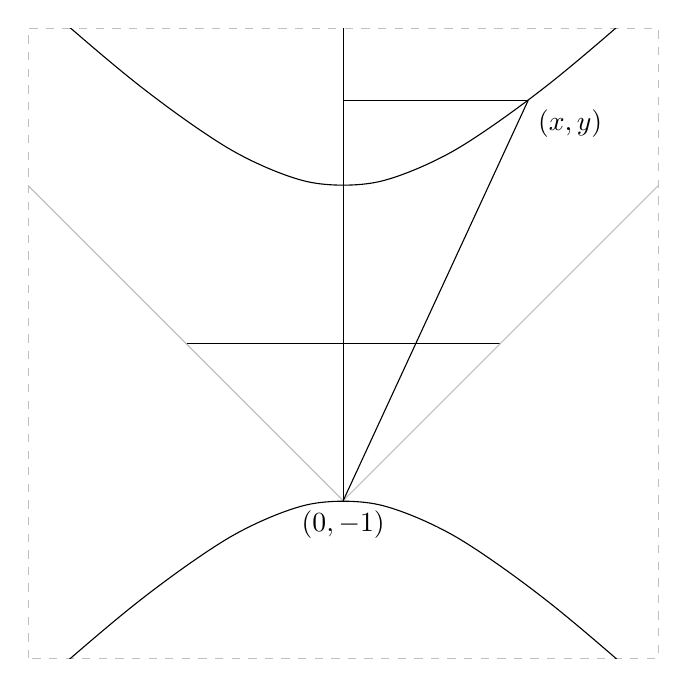
\begin{tikzpicture}[scale=2]
      \draw[dashed,lightgray] (-2,-2) rectangle (2,2);
      \clip (-2,-2) rectangle (2,2);
      \draw (-1,0) -- (1,0);
      \draw[lightgray] (0,-1) -- +(-2,2) (0,-1) -- +(2,2);
      \draw[samples=10, domain=-2:2, smooth,variable=\t]
      plot ({sinh \t}, {cosh \t})
      plot ({sinh \t}, {-cosh \t});
      \draw (0,-1) coordinate[label=below:{\((0,-1)\)}] -- (0,2);
      \def\t{1}
      \draw (0,-1) -- ({sinh \t}, {cosh \t}) coordinate[label=below right:{\((x,y)\)}];
      \draw (0,{cosh \t}) -- ({sinh \t}, {cosh \t});
    \end{tikzpicture}
  \]
  \begin{align*}
    u&= \frac{x}{1+y} \\
    k&\define {1+y} \\
    x&= ku \\
    y &= k-1 \\
    y^2-x^2 &=1 \\
    \grayunderbrace{(k-1)^2}{k^2-2k+1} -k^2u^2 &= 1 \\
    \paren{1-u^2}k^2 - 2k\cancel{+ 1} &= \cancel 1 \\
    k &= \frac{2}{1-u^2} \\
    \begin{bmatrix}
      x \\ y
    \end{bmatrix}
     &=
       \frac{1}{1-u^2}
       \begin{bmatrix}
         2u \\
         u^2+1
       \end{bmatrix}
    \intertext{Combine with the sphere's equation}
    \begin{bmatrix}
      x \\ y
    \end{bmatrix}
     &=
       \frac{1}{1\pm u^2}
       \begin{bmatrix}
         2u \\
         u^2\mp 1
       \end{bmatrix}
  \end{align*}
  \[
    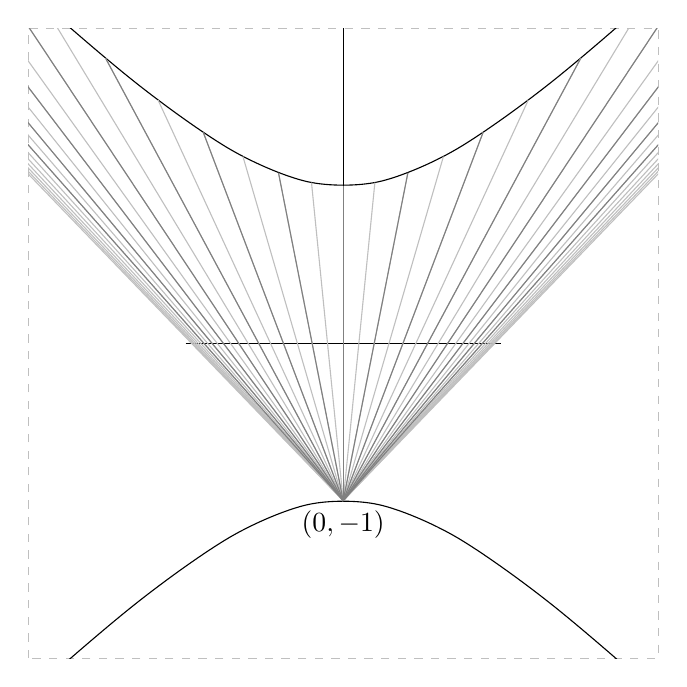
\begin{tikzpicture}[scale=2]
      \draw[dashed,lightgray] (-2,-2) rectangle (2,2);
      \clip (-2,-2) rectangle (2,2);
      \draw (-1,0) -- (1,0);
      \draw[samples=10, domain=-2:2, smooth,variable=\t]
      plot ({sinh \t}, {cosh \t})
      plot ({sinh \t}, {-cosh \t});
      \draw (0,-1) coordinate[label=below:{\((0,-1)\)}] -- (0,2);
      \foreach\t in {0,.2,...,4}
      \draw[lightgray] (0,-1) -- ({sinh \t}, {cosh \t})
       (0,-1) -- ({sinh(- \t)}, {cosh (-\t)})
      ;
      \foreach\t in {0,.4,...,3}
      \draw[gray] (0,-1) -- ({sinh \t}, {cosh \t})
       (0,-1) -- ({sinh(- \t)}, {cosh (-\t)})
      ;
    \end{tikzpicture}
  \]
  \subsection{Hyperbolic angles}
  Let \(j^2=1\). Because \(\paren{t+jx}^* = t-jx\),
  \[
    \abs{t+jx}^2 \define \paren{t+jx}^*\paren{t-jx} = t^2 -x^2
  \]
  which is proper time.

  The main trig identities:
  \begin{align*}
    \abs{e^{jt}} &=1 \\
    \cosh^2t - \sinh^2 t &= 1 \\
    e^{j\paren{\alpha+\beta}} &= e^{j\alpha }e^{j\beta} \\
    c_{\alpha+\beta}  + js_{\alpha+\beta} &= \paren{c_\alpha + j s_\alpha}\paren{c_\beta + j s_\beta} \\
    &= c_\alpha c_\beta +s_\alpha s_\beta + j\paren{c_\alpha s_\beta + s_\alpha c_\beta} \\
    c_2+js_2  &= \paren{c^2+s^2} + j\paren{2cs} \\
    \cosh 2t &= 2\cosh^2 t  -1
  \end{align*}

  Angle, arclength, area
  \begin{align*}
    \gamma(t) &\define e^{jt} \\
    \abs{\gamma(t)}^2 &= e^{jt}e^{-jt} = 1 \\
    \dot\gamma(t) &= je^{jt}
\shortintertext{gives the identities}
    \shortintertext{has arclength}
    \int \sqrt{-\abs{\dot \gamma(t)}} dt &= \int dt \\
    &=\Delta t
  \end{align*}
  \[
    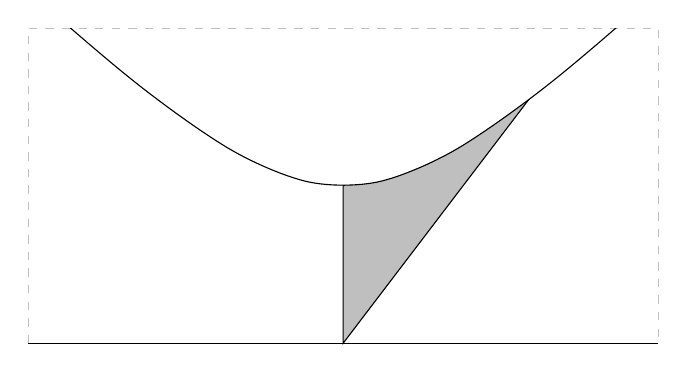
\begin{tikzpicture}[scale=2]
      \draw[dashed,lightgray] (-2,0) rectangle (2,2);
      \clip (-2,-.1) rectangle (2,2);
      \draw (-2,0) -- (2,0);
      \def\X{sinh 1}
      \def\Y{cosh 1}
      \begin{scope}
        \clip[samples=10, domain=-2:2, smooth,variable=\t]
        plot ({sinh \t}, {cosh \t}) (-2,-2) rectangle (2,2);
        \draw[fill=lightgray] (0,0) -- (\X,\Y) -- (0,1) -- cycle ;
      \end{scope}
      \draw[samples=10, domain=-2:2, smooth,variable=\t]
      plot ({sinh \t}, {cosh \t});
    \end{tikzpicture}
  \]
 Using cross products:
  \[
    \begin{array}{c|cc}
      \cdot & \gamma        & j \delta      \\
      \hline
      \alpha  & \alpha\gamma  & j\alpha\delta  \\
      -j\beta & -j\beta\gamma & -\beta\delta
    \end{array}
    \implies u^*v = u\cdot v + j u\times v
  \]
  \begin{align*}
    A&=\int \frac{e^{jt}\times j e^{jt}}2= \Im\int \frac{je^{-jt}e^{jt}}{2} \\
     &= \int \frac{1}{2} dt = \frac{\Delta t}2
  \end{align*}
\end{multicols*}
\end{document}
